\documentclass[class=minimal,border=1cm]{standalone}

\usepackage[svgnames]{xcolor}
\usepackage{tikz}
\usetikzlibrary{arrows,fit,positioning,shapes.arrows, shapes.geometric}
\usepackage{adjustbox}

\begin{document}

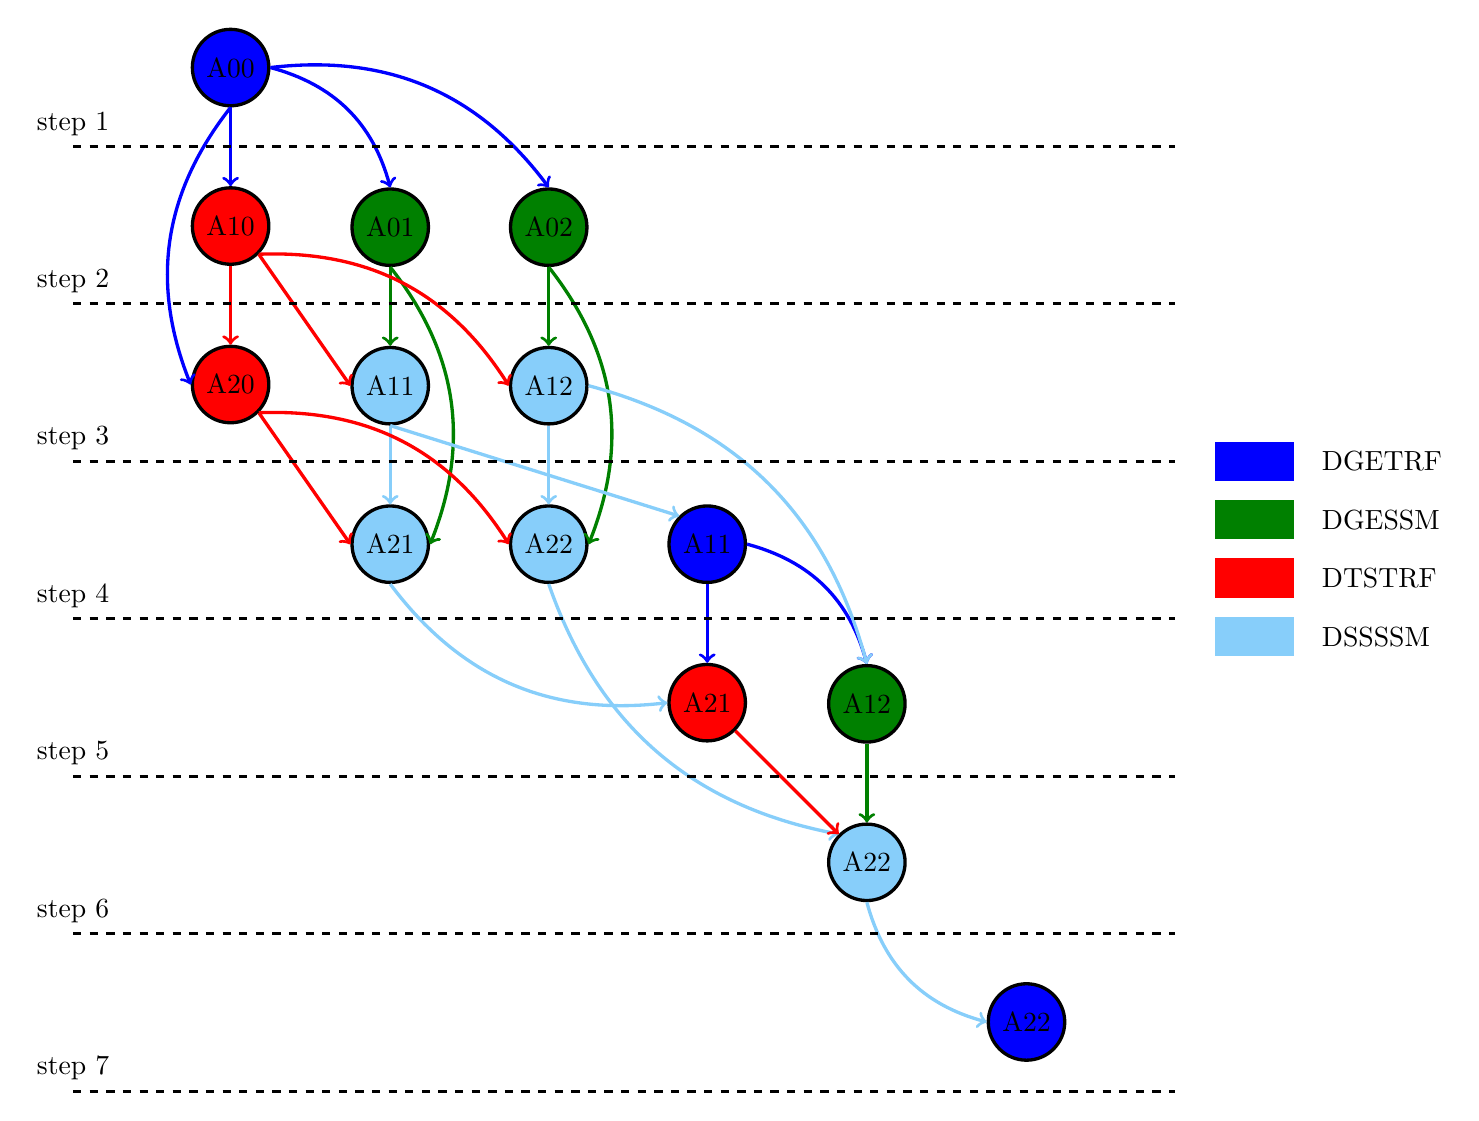
\begin{tikzpicture}[very thick,
task/.style={draw, circle, minimum width=0.5cm},
placeholder/.style={circle, minimum width=1cm},
legend/.style={draw=none, rectangle, minimum width=1cm, minimum height=0.5cm}]

	\node[task, fill=Blue] (dgetrf_A00) {A00};
	\node[placeholder, right=1cm of dgetrf_A00] (ph0) {};
	\node[task, fill=Green, below=1cm of ph0] (dgessm_A01) {A01};
	\node[task, fill=Green, right=1cm of dgessm_A01] (dgessm_A02) {A02};
	\node[task, fill=Red, below=1cm of dgetrf_A00] (dtstrf_A10) {A10};
	\node[task, fill=Red, below=1cm of dtstrf_A10] (dtstrf_A20) {A20};
	\node[task, fill=LightSkyBlue, below=1cm of dgessm_A01] (dssssm_A11) {A11};
	\node[task, fill=LightSkyBlue, below=1cm of dssssm_A11] (dssssm_A21) {A21};
	\node[task, fill=LightSkyBlue, below=1cm of dgessm_A02] (dssssm_A12) {A12};
	\node[task, fill=LightSkyBlue, below=1cm of dssssm_A12] (dssssm_A22) {A22};

	\node[task, fill=Blue, right=1cm of dssssm_A22] (dgetrf_A11) {A11};
	\node[placeholder, right=1cm of dgetrf_A11] (ph1) {};
	\node[task, fill=Green, below=1cm of ph1] (dgessm_A12) {A12};
	\node[task, fill=Red, below=1cm of dgetrf_A11] (dtstrf_A21) {A21};
	\node[task, fill=LightSkyBlue, below=1cm of dgessm_A12] (dssssm_A22_2) {A22};

	\node[placeholder, right=1cm of dssssm_A22_2] (ph2) {};
	\node[task, fill=Blue, , below=1cm of ph2] (dgetrf_A22) {A22};
	

	\path[->, color=Blue, bend left] (dgetrf_A00.east) edge (dgessm_A01.north);
	\path[->, color=Blue, bend left] (dgetrf_A00.east) edge (dgessm_A02.north);
	\path[->, color=Blue] (dgetrf_A00.south) edge (dtstrf_A10.north);
	\path[->, color=Blue, bend right] (dgetrf_A00.south) edge (dtstrf_A20.west);
	\path[->, color=Red] (dtstrf_A10.south) edge (dtstrf_A20.north);
	\path[->, color=Green] (dgessm_A01.south) edge (dssssm_A11.north);
	\path[->, color=Green, bend left] (dgessm_A01.south) edge (dssssm_A21.east);
	\path[->, color=Green] (dgessm_A02.south) edge (dssssm_A12.north);
	\path[->, color=Green, bend left] (dgessm_A02.south) edge (dssssm_A22.east);
	\path[->, color=LightSkyBlue] (dssssm_A11.south) edge (dssssm_A21.north);
	\path[->, color=LightSkyBlue] (dssssm_A12.south) edge (dssssm_A22.north);
	\path[->, color=Red] (dtstrf_A10.south east) edge (dssssm_A11.west);
	\path[->, color=Red, bend left] (dtstrf_A10.south east) edge (dssssm_A12.west);
	\path[->, color=Red] (dtstrf_A20.south east) edge (dssssm_A21.west);
	\path[->, color=Red, bend left] (dtstrf_A20.south east) edge (dssssm_A22.west);

	\path[->, color=LightSkyBlue] (dssssm_A11.south) edge (dgetrf_A11.north west);
	\path[->, color=Blue, bend left] (dgetrf_A11.east) edge (dgessm_A12.north);
	\path[->, color=Blue] (dgetrf_A11.south) edge (dtstrf_A21.north);
	\path[->, color=LightSkyBlue, bend left] (dssssm_A12.east) edge (dgessm_A12.north);	
	\path[->, color=LightSkyBlue, bend right] (dssssm_A21.south) edge (dtstrf_A21.west);	
	\path[->, color=LightSkyBlue, bend right] (dssssm_A22.south) edge (dssssm_A22_2.north west);	
	\path[->, color=Green] (dgessm_A12.south) edge (dssssm_A22_2.north);	
	\path[->, color=Red] (dtstrf_A21.south east) edge (dssssm_A22_2.north west);	

	\path[->, color=LightSkyBlue, bend right] (dssssm_A22_2.south) edge (dgetrf_A22.west);

	%auxilary lines
	\draw[dashed] (-2,-1) node[above] {step 1} -- (12, -1);
	\draw[dashed] (-2,-3) node[above] {step 2} -- (12, -3);
	\draw[dashed] (-2,-5) node[above] {step 3} -- (12, -5);
	\draw[dashed] (-2,-7) node[above] {step 4} -- (12, -7);
	\draw[dashed] (-2,-9) node[above] {step 5} -- (12, -9);
	\draw[dashed] (-2,-11) node[above] {step 6} -- (12, -11);
	\draw[dashed] (-2,-13) node[above] {step 7} -- (12, -13);

	\node[legend, fill=Blue] at (13, -5) (dgetrf_leg) {};
	\node[legend, fill=Green, below=0.2cm of dgetrf_leg] (dgessm_leg) {};
	\node[legend, fill=Red, below=0.2cm of dgessm_leg] (dtstrf_leg) {};
	\node[legend, fill=LightSkyBlue, below=0.2cm of dtstrf_leg] (dssssm_leg) {};
	\node[right=0.2cm of dgetrf_leg] {DGETRF};
	\node[right=0.2cm of dgessm_leg] {DGESSM};
	\node[right=0.2cm of dtstrf_leg] {DTSTRF};
	\node[right=0.2cm of dssssm_leg] {DSSSSM};

\end{tikzpicture}

\end{document}
